\documentclass{sig-alternate}
\usepackage{textcomp}
\usepackage{graphics}
\usepackage[latin1]{inputenc}

\hyphenation{li-neal co-rrec-ci\'on}

\begin{document}

\title{Redes Neuronales Multicapa}
\subtitle{Sistemas de Inteligencia Artifical - ITBA}

\numberofauthors{3}

\author{
	\alignauthor{Carlos Sessa}\\
	\alignauthor{Lucas Pizzagalli}\\
	\alignauthor{Nicol\'as Purita}\\	
}

\date{19 de Abril de 2012}

\maketitle

\begin{abstract}
	Se implement\'o una red neuronal supervisada multicapa para resolver los siguientes problemas:
	\begin{enumerate}
 		\item \textbf{Paridad} \label{parity}
		\item \textbf{Simetr\'ia}	\label{symmetric}
	\end{enumerate}
	Ambos problemas poseen una entrada de $N$ bits, con $2 \leq N \leq 5$.
\end{abstract}

\section*{Desarrollo}
	Las entradas para estos problemas son todas las combinaciones posibles de un arreglo de \textit{N} bits y la salida esperada es representada como un bit. Este bit se enciende cuando se cumple la condici\'on de simetr\'ia o paridad seg\'un que funci\'on l\'ogica se desee probar. \\
	Se corren distintos experimentos, variando par\'ametros y arquitecturas con el fin de lograr disminuir el tiempo de entrenamiento para la red neuronal implementada. \\
	Dada que la salida es binaria, se utilizaron distintas funciones de activaci\'on en distintas capas. En la capa oculta se utiliza una funci\'on de activaci\'on \textit{no lineal} y en la \'ultima capa, la de salida, se utiliza un funci\'on \textit{lineal}. La arquitectura elegida, con el criterio de mejor performance a la hora de entrenarla, es de $N$ entradas, $N$ neuronas en la primer capa oculta y una \'unica neurona en la capa de salida. Esta arquitectura se acomoda correctamente a los problemas \ref{parity} y \ref{symmetric}. \\
	Cabe destacar que al hacer las pruebas encontramos redes de menor
	tama\~no que resolv\'ian el problema.
	Por ejemplo, si usamos $N = 5$, el problema se puede resolver con
	$N-2$ neuronas en la capa oculta. Dado que poder elegir un n\'umero
	de neuronas menor a $N$ es posible pero no se cumple para todos
	los $N$ preferimos hacer las pruebas correspondientes con $N$ neuronas
	en la capa oculta.


\section*{Resultados obtenidos}

	En la figura \ref{fig:symN5} se puede ver como utilizando la tangente hiperb\'olica como funci\'on de activaci\'on para el problema de la \textit{Simetr\'ia} se logra un mejor error que utilizando la exponencial.\\
	En la figura \ref{fig:parN5} se puede observar como el problema de \textit{Paridad} utilizando la funci\'on de activaci\'on exponencial no se llega a entrenar la red con un error menor al deseado, \textit{0.01}, en un lapso de 5000 \'epocas a diferencia de la funci\'on tangencial, donde la red logra entrenarse en 1487 \'epocas. El motivo por el cual la funci\'on de activaci\'on exponencial no termina en 5000 \'epocas es porque no se realiza ninguna correcci\'on de los pesos ya que es 0 el valor de la funci\'on. \\
	Como se observa en las figuras \ref{fig:tanhAllVsLinealLast} y \ref{fig:tanhAllVsLinealLastSymetric} al poner una funci\'o lineal en la \'ultima capa la red es entrenada en menos tiempo, es decir en menos \'epocas. Esto se debe a que en la \'ultima capa la estructura de la red se comporta como un perceptron simple y el problema en ese nivel es linealmente separable. Por este motivo es mejor utilizar una funci\'on \textit{lineal} frente a una \textit{no-lineal}.\\

\section*{Conclusiones}

	La primera es que, dado que la salida de la red es binaria, podemos mejorar el tiempo de entrenamiento poniendo una funci\'on de activaci\'on \textit{escal\'on} en la capa de salida. Para aplicar esto debemos realizar la transformaci\'on de la entrada de mapear los $0$ al $-1$.\\
	El segundo punto a destacar es el peso de la aleatoriedad de los pesos. Por ejemplo, notamos que poniendo distintas semillas se puede lograr que la red con $N=2$ tarde menos en entrenarse que con $N=5$.\\
	El \'ultimo punto a destacar es la imposibilidad de entrenar la red con funciones de activaci\'on \textit{escal\'on} y \textit{no-lineal} durante su entrenamiento. El motivo por el cual la red no puede ser entrenada con estas funciones es que el problema \textbf{no} es \textit{linealmente separable}.
	Este es el motivo por el cual se dicide comparar en las figuras las funciones de activaci\'on \textit{sigmoidea} y \textit{exponencial} ya que son las \'unicas funciones que resultan correctas para el entrenamiento de la red neuronal.

\newpage

\begin{figure}[!ht]
	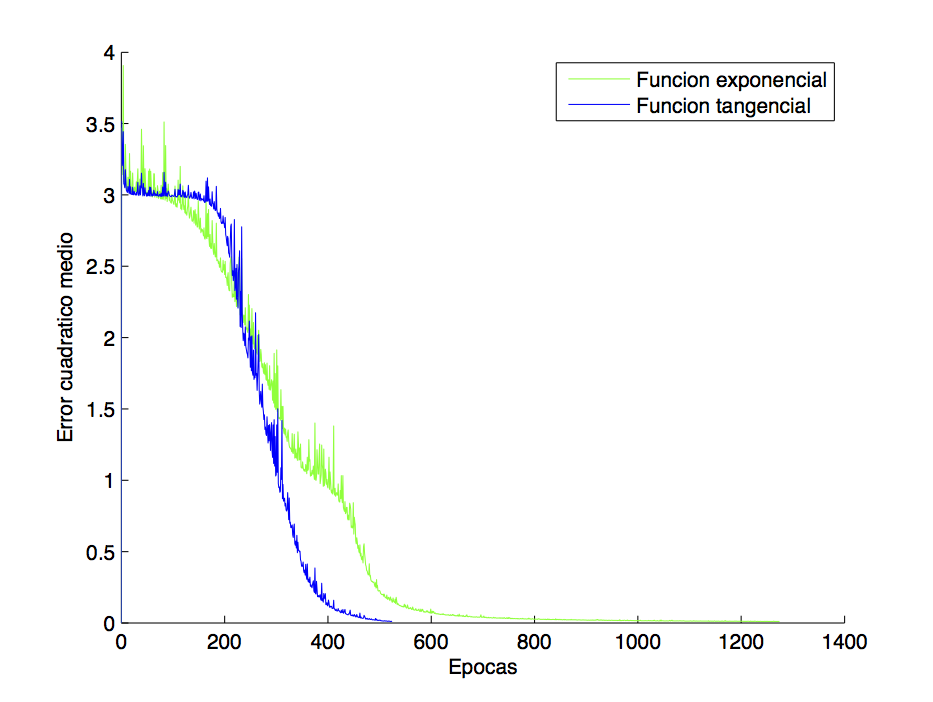
\includegraphics[scale=0.5]{./images/tanhVsExp.png}
  \caption{Comparaci\'on del error para distintas funciones de activaci\'on con $N = 5$ en el problema de Simetr\'ia}
  \label{fig:symN5}
\end{figure}

\begin{figure}[!ht]
	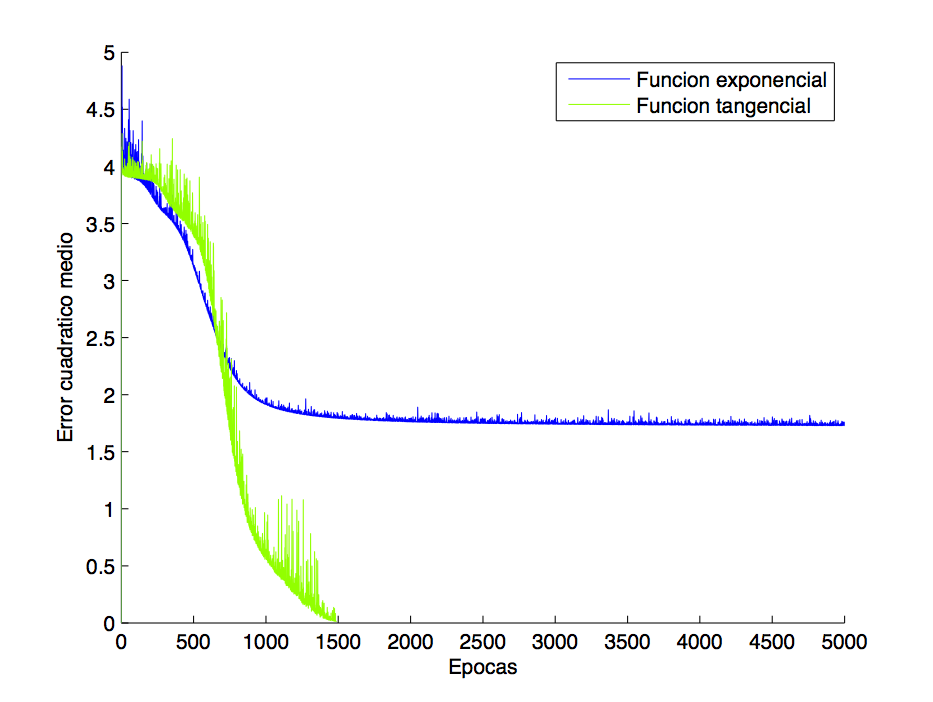
\includegraphics[scale=0.5]{./images/tanhVsExpParity.png}
  \caption{Comparaci\'on del error para distintas funciones de activaci\'on con $N = 5$ en el problema de Paridad}
  \label{fig:parN5}
\end{figure}

\begin{figure}[!ht]
	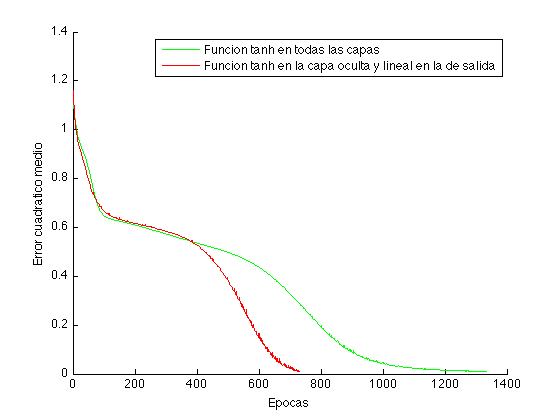
\includegraphics[scale=0.5]{./images/tanhAllVsTanhAndLineal.png}
  \caption{Comparaci\'on del error para distintas funciones de activaci\'on en la \'ultima capa, con $N = 3$ en el problema de Paridad}
  \label{fig:tanhAllVsLinealLast}
\end{figure}


\begin{figure}[!ht]
	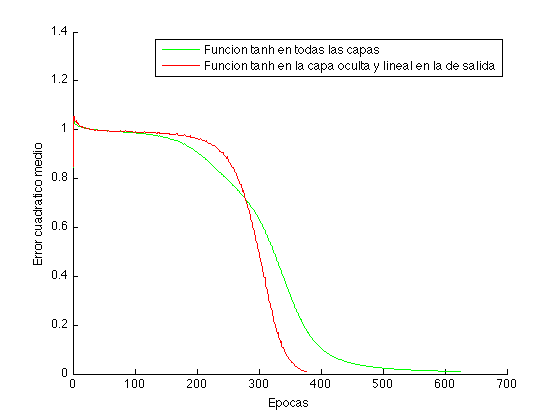
\includegraphics[scale=0.5]{./images/tanhAllVsTanhAndLinealSymetric.png}
  \caption{Comparaci\'on del error para distintas funciones de activaci\'on en la \'ultima capa, con $N = 3$ en el problema de Simetr\'ia}
  \label{fig:tanhAllVsLinealLastSymetric}
\end{figure}

\end{document}